\subsection{Target Tracking Video Stabilization}
\label{sec:stabilization}
Video stabilization is a family of techniques used to reduce blurring associated with the motion of the camera  during exposure, and it generally compensates for pan and tilt of the camera, although rotations can also be compensated.\\

\noindent The main idea of Target Tracking Video Stabilization \footnote{\url{https://es.mathworks.com/help/vision/examples/video-stabilization.html}} is to use a block-based parametric motion model to correct translational and rotational camera motions. We define the target to track (in our system a square area in the lower left corner) and we establish a dynamic search region, whose position is determined by the last known target location. Then, we search for the target only within this search region. In each subsequent video frame we determine how much the target has moved relative to the previous frame, and we use this information to remove unwanted translational camera motions and generate a stabilized video. Notice that we add a black padding to all the frames to deal with the loss of information in the borders after stabilization, and we apply the same stabilization and padding to the ground truth for evaluation.

\begin{figure}[h]
\centering
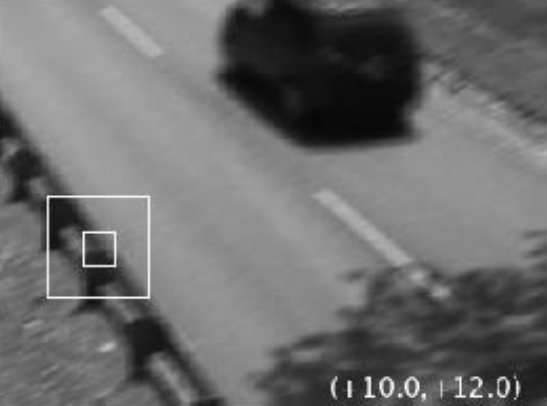
\includegraphics[width=105pt, height=95pt]{figures/target_tracking.png} 
\caption{Target Tracking Video Stabilization frame. The square on the left bottom area denotes the area to track used by the stabilization algorithm.}
\label{fig:fg}
\end{figure}